\documentclass[12pt, letterpaper]{article}
\usepackage[utf8]{inputenc}
\usepackage{graphicx}
\usepackage{amsmath}
\usepackage{tabularx}
\usepackage{tikz}
\usepackage{hyperref}
\usepackage[ruled, noline, noend]{algorithm2e}

\usetikzlibrary{calc}
\graphicspath{{images/}}

\newcommand{\minus}{\scalebox{0.75}[1.0]{$-$}}

\hypersetup{colorlinks=true, urlcolor=cyan}

\title{Network Flow}
\author{Mikhail Mints}
\date{April 16, 2020} %PUT ACTUAL DATE

\begin{document}

\maketitle

\section{Introduction}
Network flow algorithms are very useful in many different types of problems, and have a lot of applications. They appear somewhat frequently in USACO and other programming contests. In this lecture, we will be discussing how network flow works and some algorithms and ideas related to it.

\section{Flow Networks}
The most intuitive way of thinking about a flow network is this: We have a system of pipes (edges) that are connected to each other in junctions (nodes). Each pipe has a certain \textbf{capacity} - which could be thought of as the maximal amount of water that can flow through the pipe (in a certain time). The pipes are directed, each flowing from one node to another. There exist 2 special nodes, called the \textbf{source} ($s$) and the \textbf{sink} ($t$). The  water flows out of the source, travels through the system of pipes, and flows into the sink. Each pipe has a certain \textbf{flow} going through it, not greater than its capacity. For each node other than the source and the sink, the total inflow equals the total outflow, meaning that the sum of flows in incoming pipes equals the sum of flows in outgoing pipes.

\newpage
We can represent such a network using a weighted directed graph, for example:

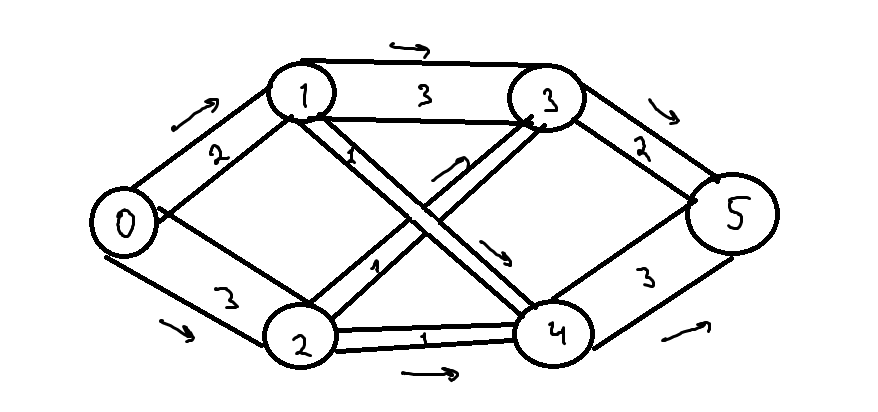
\includegraphics[scale=0.5]{figure1.png}

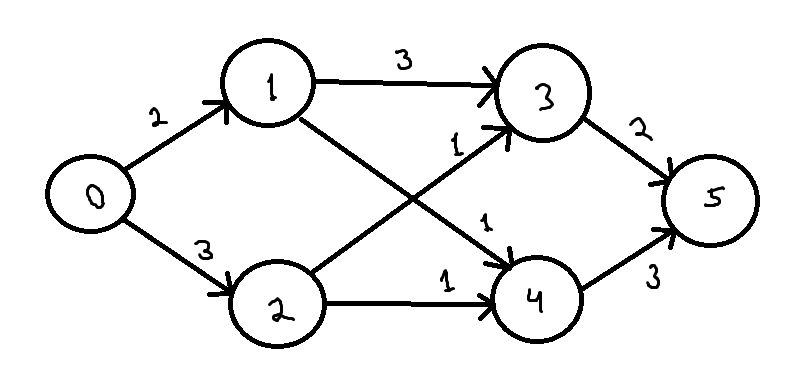
\includegraphics[scale=0.5]{figure2.png}

Each of the edges in the graph above represents a pipe, and its weight is its capacity.

(Note that this particular network flow example used throughout the lecture was taken from \textit{Algorithms} by Sedgewick and Wayne.)

\section{The Max-Flow Problem}
The statement of the max-flow problem is the following: Given a network with a source node $s$ and a sink node $t$, find a way to distribute the flow among the pipes that maximizes the total flow from $s$ to $t$.

\subsection{Simple, Incorrect Solution}
Suppose we have a path from $s$ to $t$. The most flow that we can add is the minimum of the (remaining) capacities along this path. A simple approach would be to find possible paths from $s$ to $t$ and add the maximum possible flow to each of the paths. For the above network, if node 0 is the source and node 5 is the sink, this could look something like this:

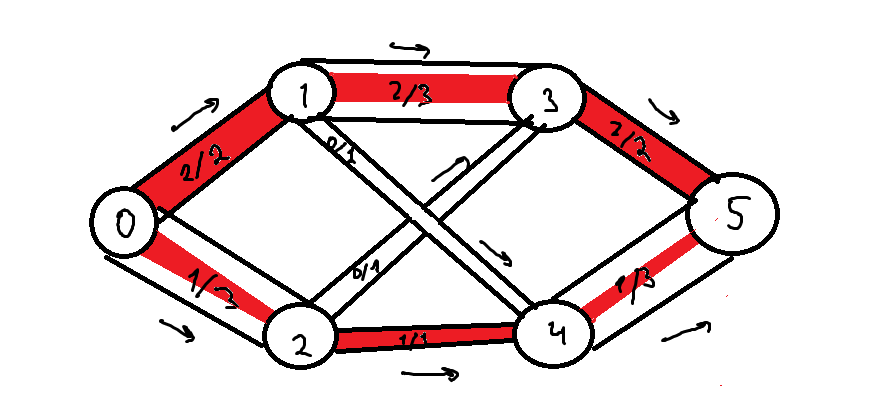
\includegraphics[scale=0.75]{figure3.png}

After filling in the flows along the two paths shown, we can't add any more flow anywhere. So our total flow is $2+1=3$. However, this is not the optimal solution! We could have actually made our flows go like this:

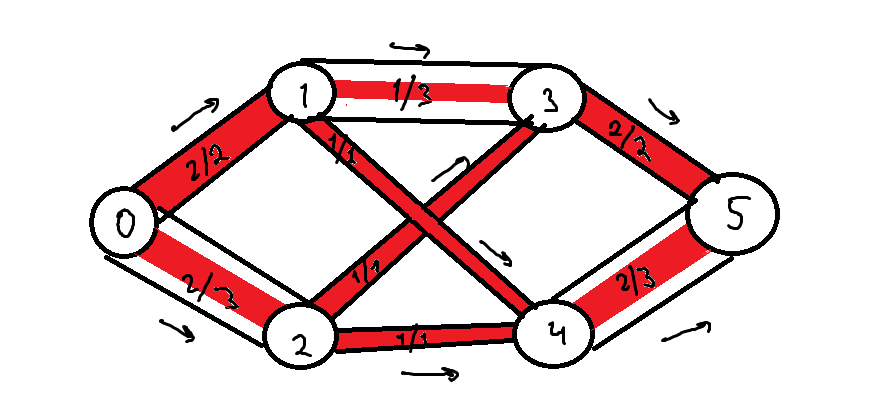
\includegraphics[scale=0.75]{figure4.png}

Here, for all the nodes, inflow still equals outflow, but the total flow is now $2+2=4$. How can we create an algorithm that solves this problem correctly?

\newpage
\section{Ford-Fulkerson Algorithm}
The \textbf{Ford-Fulkerson algorithm} is the general algorithm for solving network flow problems that can be implemented using a number of different approaches. But the general idea is based on the following:

\subsection{Augmenting Paths}
In the previous example, we looked at the directed graph representing the network and added flow to the paths leading from $s$ to $t$. We first added the path $0\rightarrow1\rightarrow3\rightarrow5$, and then we added the path $0\rightarrow2\rightarrow4\rightarrow5$, after which we couldn't add any more paths. But what if we allow paths whose edges can go in either direction, not just following the directed graph? If we have such a path, when we travel in the reverse direction, we could subtract flow from the edge instead of adding it. This will still conserve the property that inflow must equal outflow. Such a path is called an \textbf{augmenting path}. In the first image on the last page, we can add the following augmenting path: $0\rightarrow2\rightarrow3\rightarrow1\rightarrow4\rightarrow5$. If we add a flow of 1 along this path (subtracting in the $3\rightarrow1$ edge since it is a backward edge, we can get what we had in the second picture. We were able to add this path, because for all the forward edges had some capacity remaining, and all of the backward edges had some flow left to remove.

\subsection{The Algorithm}
The Ford-Fulkerson Algorithm is a generalized algorithm for solving the max-flow problem. It is the following:

\begin{algorithm}
\caption{Ford-Fulkerson}
Flow is initially 0 everywhere\;
\While{augmenting path exists}{
    path $\leftarrow$ findAugmentingPath()\;
    \For{$v$ in path}{
        Increase flow as much as possible;
    }
}
\end{algorithm}
Since each time we are adding a new augmenting path, we are adding at least 1 unit of flow, the algorithm will eventually terminate at the maximum flow.

\section{More Specific Algorithms}

\subsection{Residual Network}
How do we actually find an augmenting path in a flow network? There exist several ways to do that. Most of them use the idea of a \textbf{residual network}. A residual network is a way of representing the network with the addition of flows in a way that can help us find new augmenting paths. For each edge $e=(u, v)$ in the network with flow $f_e$ and capacity $c_e$, in the residual network we have an edge $(u, v)$ with capacity $c_e-f_e$, and an edge $(v, u)$ with capacity $f_e$. In other words, the forward edge represents the remaining capacity and the backward edge represents the flow. Here is an example for the first image on page 3:

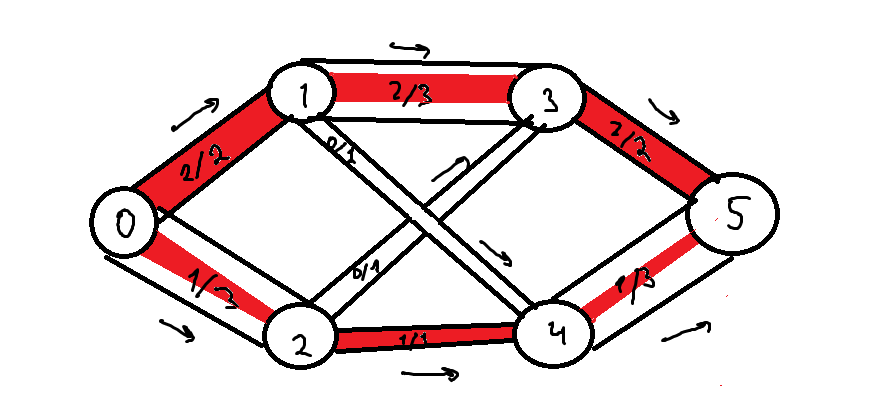
\includegraphics[scale=0.35]{figure3.png}
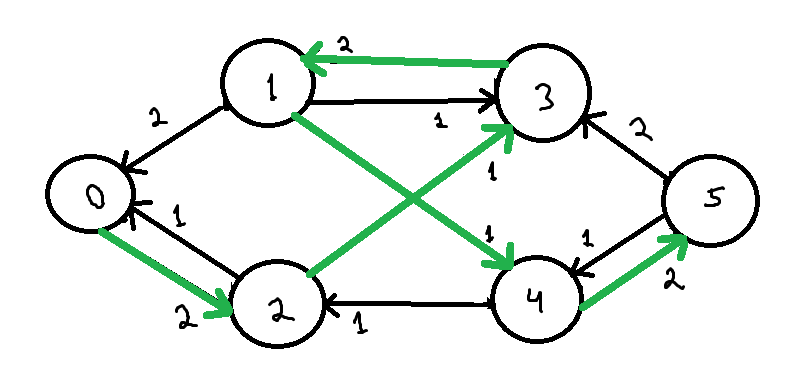
\includegraphics[scale=0.35]{figure5.png}

As you can see in the above image, some pairs of nodes have 2 edges, and the capacity of the edge going in the backward direction represents the amount of flow. The edges highlighted in green represent the augmenting path that needs to be added to this network in order to transform it into the correct solution.

The reason that we are doing this is because now, when we look at a path in the residual network, when we are adding flow, we can subtract it from the capacity of the edge and add it to the edge going in the opposite direction. If we were originally going in the forward direction (with the direction of the original network), we are reducing the capacity and adding flow. If we were going in the backward direction (against the direction of the original network), we are reducing the flow and adding new capacity. So we don't have to worry about whether the edge we are traversing is forward or backward - we do the same procedure for both.

\newpage
\subsection{Edmonds-Karp Algorithm}
The \textbf{Edmonds-Karp algorithm} is a specific implementation of the Ford-Fulkerson algorithm, in which the next augmenting path found is the shortest path. We can do this by performing a BFS in the residual network. After we find an augmenting path, we find the amount of flow that can be added along the path, and update the weights of the forward and backward edges in the path. This implementation has a runtime of $O(VE^2)$

In another version of this algorithm, instead of finding the shortest path, we could find the path that has the maximum capacity. That can be done using a modified version of Dijkstra's algorithm - you can find this version described in more detail in the USACO Training pages.

\section{Other Max-Flow Algorithms}
\subsection{Push-Relabel}
The push-relabel algorithm is a different max-flow algorithm that is more efficient than Ford-Fulkerson. It has a complexity of $O(V^2E)$, with some variants that are more efficient. Instead of adding augmenting paths to the whole network, this algorithm starts with a pre-flow that does not necessarily balance the inflow and outflow of each node. Then it applies certain "push" and "relabel" operations that can move the flow between the nodes in order to convert it into the max-flow. You can look at some of the past lectures or other online resources if you are interested in learning more about how this works.

\subsection{Linear Programming}
The max-flow problem can actually be expressed as a linear programming problem. Our variables are the flows going through each edge of the network, and our goal is to maximize the sum of the flows going into the sink subject to the constraints that each flow must not exceed the capacity of the edge, and that the inflow and outflow of each node must be equal. This means that we can use the simplex algorithm and other techniques mentioned in the Linear Programming lecture in order to solve the max-flow problem.

\newpage
\section{The Min-Cut Problem}
We can define an \textbf{$st$-cut} of a network as a partition of the nodes into 2 groups, one containing $s$ and the other containing $t$. To create this partition, we need to remove certain edges from the network - this is the cut. Our goal is to minimize the total capacity of the cut.

\subsection{Maxflow-Mincut Theorem}
Even though the min-cut problem doesn't seem very similar to the max-flow problem, they are actually very closely related. The \textbf{maxflow-mincut theorem} simply states that for any flow network, the maximum flow equals the minimum cut. This means that we can actually use the Ford-Fulkerson algorithm to compute the minimum cut.

After running the Ford-Fulkerson algorithm on a network, it is also possible to find the actual edges that correspond to the min-cut. At the end of the algorithm, no more augmenting paths exist between the source and the sink. We can actually use the final residual network to find all the nodes that are reachable from the source. Those nodes will be on the same side of the cut as the source node. In order to find the edges to cut, we look at all the connections between the nodes in this group and those that aren't reachable through the residual network.

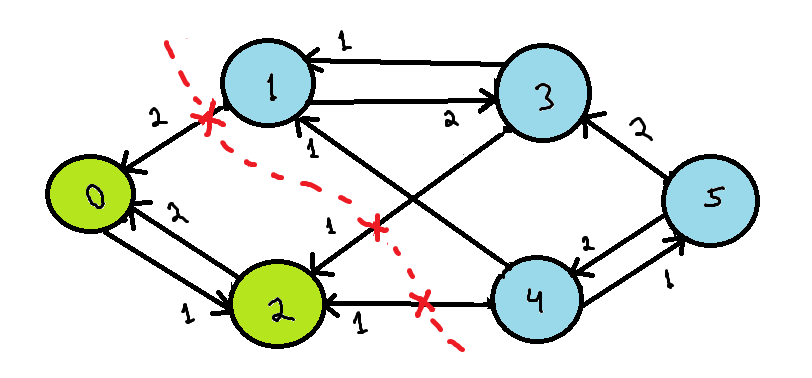
\includegraphics[scale=0.75]{figure6.png}

Here you can see the final residual network (produced by adding flow along the green path in the image on page 5). In green are the nodes reachable from the source, and in blue are the nodes reachable from the sink. The red line that divides them is the minimum cut, with a cost of 4.

\section{Bipartite Matching}
Another common application of max-flow algorithms is \textbf{bipartite matching}. Suppose we are given two groups, $A$ and $B$. Only certain pairs are possible, for example $A_1$ can be paired with $B_2$ and $B_3$, $A_3$ can be paired with $B_2$ and $B_4$, etc. Our goal is to find a matching between $A$ and $B$ so that we have the maximum possible number of pairs. In order to do this, we can build a flow network like this:

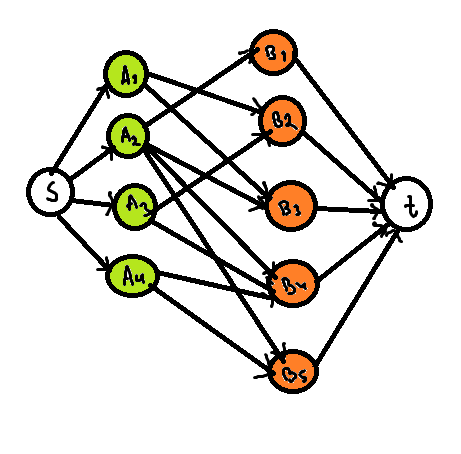
\includegraphics[scale=0.75]{figure7.png}

We added a source node that is connected to all the $A$ nodes and a sink node that is connected to all the $B$ nodes. All the edges have a capacity of 1. If we run a max-flow algorithm on this network, the flow will be equal to the number of matched pairs, and it will be going along the edges corresponding to the chosen pairs.

\section{Problems}
\begin{itemize}
    \item Drainage Ditches (USACO Training 4.2)
    \item Telecowmunication (USACO Training 5.4)
    \item \href{http://www.usaco.org/index.php?page=viewproblem2&cpid=93}{Cow Steeplechase (USACO 2011)}
    \item \href{https://codeforces.com/problemset/problem/808/F}{Card Game (Codeforces)}
    \item \href{https://codeforces.com/contest/1404/problem/E}{Bricks (Codeforces)}
\end{itemize}

\section{References}
\begin{itemize}
    \item \parbox{350pt}{\textit{Algorithms} by Robert Sedgewick and Kevin Wayne}
    \item \parbox{350pt}{\href{https://train.usaco.org}{USACO Training Pages: Network Flow Algorithms}}
    \item \parbox{350pt}{\href{https://en.wikipedia.org/wiki/Ford-Fulkerson_algorithm}{Wikipedia - Ford-Fulkerson algorithm}}
    \item \parbox{350pt}{\href{https://activities.tjhsst.edu/sct/lectures/1920/2020_4_30_Flow.pdf}{Previous lecture by Udbhav Muthakana}}
\end{itemize}

\end{document}